% Let the points be
% \begin{align}
% \myvec{x_1\\y_1} = \myvec{a \\0}  ; \myvec{x_2\\y_2}  = \myvec{0\\ 2a}; \myvec{x_3\\y_3} =  \myvec{2a \\a}\label{2/4/2/1.0.1} 
% \end{align}
% In order to convert to rectangular coordinate system, the y-axis should be rotated by $30^{\degree}$ in anti-clockwise.
% Transformed coordinates of \myvec{x_1\\y_1}, \myvec{x_2\\y_2} \& \myvec{x_3\\y_3} be \myvec{x_4\\y_4}, \myvec{x_5\\y_5} \& \myvec{x_6\\y_6} respectively.\\
% \begin{align}
%    x_4 = OX_1 + X_1X_4 &= x_1+y_1\cos{60^{\degree}}\\
%    y_4 = OY_1\cos{30^{\degree}}&= y_1\cos{30^{\degree}}  
% \end{align}
% \begin{align}
% \myvec{x_4\\y_4} = \myvec{1 \ \cos{60^{\degree}} \\ 0 \  \cos{30^{\degree}}} \myvec{x_1\\y_1}\label{2/4/2/eq:1.0.2}   
% \end{align}
The generalised equation for transformed coordinates $\myvec{x_t\\y_t}$ when the angle between axes $\theta$ is,
\begin{align}
\vec{x}_t = \vec{T}  \vec{x} \label{2/4/2/eq:1.0.3}  
\end{align}
%
where
\begin{align}
\vec{T} = \myvec{1  &  \cos \theta\\ 0 & \sin \theta} \vec{x}
\end{align}
% Let the transformed point be $\vec{X_t}$, $\vec{T}$ be the transformation matrix and the point in angular axes be $\vec{X}$, \eqref{2/4/2/eq:1.0.3} can be written as 
% \begin{align}
%  \vec{X_t} = \vec{T} \ \vec{X}\label{2/4/2/eq:1.1.5}  
% \end{align}
Thus, using \eqref{2/4/2/eq:1.0.3}, the equivalent rectangular coordinates for the given point are 
 \begin{align}
  \vec{x}_1 = \myvec{a\\0}, \vec{x}_2 = \myvec{a\\\sqrt{3}a}, \vec{x}_3 =\myvec{\frac{5a}{2}\\\frac{\sqrt{3}a}{2}} \label{2/4/2/eq:1.0.5}    
 \end{align}
The distance between the points is 
\begin{align}
d_{ij} &= \norm{\vec{x}_{ti}-\vec{x}_{tj}} \label{2/4/2/eq:1.1.7}
% \end{align}
% Substituting \eqref{2/4/2/eq:1.1.5} in \eqref{2/4/2/eq:1.1.7},
% \begin{align}
\\
& = \norm{\vec{T}\vec{x}_{i}-\vec{T}\vec{x}_{j}} \label{2/4/2/eq:1.1.8}
% \end{align}
% \begin{align}
\\
& = \norm{\vec{T}\brak{\vec{x}_{i}-\vec{x}_{j}}} \label{2/4/2/eq:1.1.123}
% \end{align}
% \begin{align}
\\
&= \sqrt{\brak{\vec{x}_{i}-\vec{x}_{j}}^\top \vec{T}^\top\vec{T}\brak{\vec{x}_{i}-\vec{x}_{j}}}  \label{2/4/2/eq:1.1.9}
\end{align}
Substituting numerical values, 
\begin{align}
d_{ij} = \sqrt{3}a \\
\end{align}
% Therefore,
% \begin{align}
%     d_{12}=d_{23}=d_{31}    \label{2/4/2/eq:1.1.13}
% \end{align}
% From \eqref{2/4/2/eq:1.1.13} 
and the three points form an equilateral triangle
%\counterwithin{figure}{section}
% \begin{figure}[!ht]
% 	\centering
% 	\includegraphics[width=\columnwidth]{BOP1.jpg}
% 	\caption{Points defined on angular \& rectangular axes}
% 	\end{figure}
%\counterwithin{figure}{section}
\begin{figure}[!ht]
    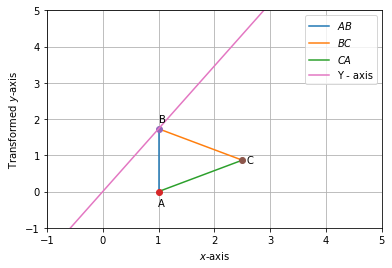
\includegraphics[width=\columnwidth]{2/solution/4/2/tri.png}
    \caption{Points plotted in Python}
    \label{2/4/2/Fig2: Points plotted in Python}
\end{figure}

